\documentclass[12pt]{report}
\usepackage[]{graphicx}\usepackage[]{color}
%% maxwidth is the original width if it is less than linewidth
%% otherwise use linewidth (to make sure the graphics do not exceed the margin)
\makeatletter
\def\maxwidth{ %
  \ifdim\Gin@nat@width>\linewidth
    \linewidth
  \else
    \Gin@nat@width
  \fi
}
\makeatother

\definecolor{fgcolor}{rgb}{0.345, 0.345, 0.345}
\newcommand{\hlnum}[1]{\textcolor[rgb]{0.686,0.059,0.569}{#1}}%
\newcommand{\hlstr}[1]{\textcolor[rgb]{0.192,0.494,0.8}{#1}}%
\newcommand{\hlcom}[1]{\textcolor[rgb]{0.678,0.584,0.686}{\textit{#1}}}%
\newcommand{\hlopt}[1]{\textcolor[rgb]{0,0,0}{#1}}%
\newcommand{\hlstd}[1]{\textcolor[rgb]{0.345,0.345,0.345}{#1}}%
\newcommand{\hlkwa}[1]{\textcolor[rgb]{0.161,0.373,0.58}{\textbf{#1}}}%
\newcommand{\hlkwb}[1]{\textcolor[rgb]{0.69,0.353,0.396}{#1}}%
\newcommand{\hlkwc}[1]{\textcolor[rgb]{0.333,0.667,0.333}{#1}}%
\newcommand{\hlkwd}[1]{\textcolor[rgb]{0.737,0.353,0.396}{\textbf{#1}}}%

\usepackage{framed}
\makeatletter
\newenvironment{kframe}{%
 \def\at@end@of@kframe{}%
 \ifinner\ifhmode%
  \def\at@end@of@kframe{\end{minipage}}%
  \begin{minipage}{\columnwidth}%
 \fi\fi%
 \def\FrameCommand##1{\hskip\@totalleftmargin \hskip-\fboxsep
 \colorbox{shadecolor}{##1}\hskip-\fboxsep
     % There is no \\@totalrightmargin, so:
     \hskip-\linewidth \hskip-\@totalleftmargin \hskip\columnwidth}%
 \MakeFramed {\advance\hsize-\width
   \@totalleftmargin\z@ \linewidth\hsize
   \@setminipage}}%
 {\par\unskip\endMakeFramed%
 \at@end@of@kframe}
\makeatother

\definecolor{shadecolor}{rgb}{.97, .97, .97}
\definecolor{messagecolor}{rgb}{0, 0, 0}
\definecolor{warningcolor}{rgb}{1, 0, 1}
\definecolor{errorcolor}{rgb}{1, 0, 0}
\newenvironment{knitrout}{}{} % an empty environment to be redefined in TeX

\usepackage{alltt}
\newcommand{\SweaveOpts}[1]{}  % do not interfere with LaTeX
\newcommand{\SweaveInput}[1]{} % because they are not real TeX commands
\newcommand{\Sexpr}[1]{}       % will only be parsed by R



\usepackage{../thesis}
\usepackage{pdflscape}
\usepackage{rotating}
\usepackage{setspace}
\usepackage[titles]{tocloft}
\renewcommand\cfttoctitlefont{\normalsize}
\setlength\cftchapindent{0pt}
\usepackage{fancyhdr}
\pagestyle{fancy}
\fancyhf{}
\cfoot{\thepage}
\fancyhead[R]{}
\renewcommand{\headrulewidth}{0pt}

%%%% smaller caption size for R plots %%%%
\usepackage[font=scriptsize]{caption}

%%%% clears notes in bibliograhpy %%%%
\AtEveryBibitem{\clearfield{note}}

\makeatletter
\newcommand\iraggedright{%
	\let\\\@centercr\@rightskip\@flushglue \rightskip\@rightskip
	\leftskip\z@skip}
\makeatother

\usepackage{titlesec}
\titlespacing*{\chapter}{0pt}{2in}{0pt}
\titleformat{\chapter}[display]{\normalfont}{\chaptertitlename\ \thechapter}{12pt}{\normalfont}
\titleformat*{\section}{\normalsize\bfseries} 
\titleformat*{\subsection}{\normalsize\itshape} 
\titlespacing*{\section}{0pt}{0ex plus 1ex minus .2ex}{0ex plus .2ex} 
\titlespacing*{\subsection}{0pt}{0ex plus 1ex minus .2ex}{0ex plus .2ex}

\renewcommand{\chaptername}{{CHAPTER}}

\title{Cracks in the foundation: The myth of Latin American national literatures}





\begin{document}


\begin{singlespace}
\chapter{ISAACS' \textit{MARÍA}}
\end{singlespace}

\section{Introduction: set up the problem}
The geographic area that today is Colombia has seldom presented itself as a unified national community. Most Spanish ex-colonies underwent many years of social, cultural, and political stratification before experiencing a national consolidation during the mid-to-late nineteenth century.While Nueva Granada and its later counterparts followed many of the broad trends associated with independence, Colombia, for several reasons, has struggled with national unification to this day.Some \enquote{foundational} works of literature in the burgeoning republics, such as José Marmol's \textit{Amalia}, deal explicitly with the socio-political challenges of a new state.On the other hand, Jorge Isaacs’ treatment of the political situation in his 1867 novel \textit{María} is less overt, some would say absent. Critics such as Doris Sommer and Sharon Magnarelli find Isaacs’ displacement of politics to be an essential part of understanding the value of his novel and its critique of nascent Colombia.Others, like Gustavo Mejía, have a parsed more nuanced connections, finding in the novel \enquote{las repercusiones de los acontecimientos que, aproximadamente en 1850, iniciaron la transformación del modo de producción heredado de la colonia, caracterizado por las prohibiciones mercantilistas para evitar el desarrollo de manufacturas nativas} \cite[262]{Mejia1976}.Sommer points out that, in her opinion, the success of Colombia's founding fiction \textit{María} as a nation-building piece of literature is somewhat of an anomaly when compared to the other novels she has examined. However, what makes \textit{María} the outlier in Sommer's study is an attempt to homogenize regional characteristics under the hypernym of \enquote{Latin America.}Isaacs does not critique social institutions in order to outline a way forward, he does not make explicit commentary in order to condemn outdated customs, he does not frame regional conflicts in order to substantiate a particular view of history. She also asserts that the disenchantment present in Isaacs' narrative also makes its successful integration into \enquote{national histories} unexpected \cite[30]{Sommer1991}.
That his novel stands out in this regard does not make it odd as a Colombian national allegory. Colombian literature embraced and grew into a pessismistic tone that has reflected its politics and remained throughout the 20th century.Conversely, the novel's international success indicates that there is something universal in it that reaches a broader audience.The fact that the novel has connected locally and globally is due to varying degrees of readerly recognition through thematic content.Most critics of Isaacs' work find in it unique analogies to the struggle of forming Colombian society; some through love, some economy, others race and Jewish heritage.Nevertheless, to be reimplemented as a successful allegory for decades after its publishing a text must continue to connect with a renewing audience. While the subject matter of the mid-1800's becomes more remote as time goes on, the stylistic features of the novel remain intact.It is this stylistic connection that has conducted many novels into the national space and more importantly allowed them to remain despite the obsolescence of their anachronistic theme and genre.
While some authors and novels have been acknowledged for connecting with an audience through form, the influence of language and structure is often overlooked.In the case of national literatures, critics like Benedict Anderson recognize that the formation of a print vernacular is essential to the formation of national communities.This is especially pertinent in the ex-Spanish colonies in the Americas given their shared administrative language. Whereas national coalescence in Europe could be drawn along linguistic lines, that was not the obvious case in the Americas. For that reason, subtler stylistic and lexical characteristics played the role of delimiting boundaries of identity through literature. \textit{María} seems anomalous precisely because of the characteristics that \textit{make} it Colombian, some thematic others stylistic.The fact that the novel stands out parallels the unique trajectory of Colombia's national history when compared to other American nations. A fact that not only highlights the regional characteristics of \textit{María} and Colombia, but the regional uniqueness of national movements throughout the Americas.


\section{Review of literature}
\subsection{General info, Plot summary}

Jorge Isaacs was born in 1837 to a Jewish English immigrant father from Jamaica and a native Colombian mother. His father began in mining and after gaining enough capital purchased several estates in the Cauca valley. Jorge Isaacs left to study in Bogotá in 1848 and returned in 1852. He actively took up arms in various regional struggles and later worked for the government in several capacities, including a member of Congress and an Ambassador to Chile. After these experiences his political allegiances shifted to radical liberalism two years after the first edition of \textit{Maria} was published in 1867. 

The protagonist of the novel, Efraín, the son of a Jewish English immigrant from Jamaica, returns to his family estate after years study in the Capital.
It is interesting to note that in the first edition Efraín spends only four years in Bogotá, a period that Isaacs changes to six years in later editions \cite[67]{Isaacs2012}. According to McGrady this made María's age, now fifteen years old, more appropriate for an engagement. A fact that highlights Isaacs awareness of the need to address an audience beyond the cultural confines of Cauca.
He finds on his return that he harbors a deep love for the novel's namesake character María.
The parents of María, relatives of Efraín's father, were also Jewish immigrants living in Jamaica.
After her mother died, her father left her and she is raised as a part of Efraín's family from her early childhood.
During Efraín's return visit his father falls ill upon receiving news of serious financial troubles.
María also suffers from a severe mysterious disease, which she has possibly inherited from her mother.
Her emotions t is decided that her love for Efraín must be tempered in order to not set off her symptoms.
Mid-way through the novel Efrain tells the lifes story of one of his family’s closest servants.
The intercalated story of Nay and Sinar recounts the parallel story of love between the children of rival tribes in West Africa.
The lovers are captured and shipped off to New Granada as slaves but Sinar is killed.
Nay survives and is discovered at the home of a slave trader by Efrain’s father who purchases her only to grant her freedom.
However Nay stays on to become the families closest servant and the children’s beloved caretaker.
The family agrees that Efraín and María will remain engaged while Efraín goes off to finish his studies in Europe.
In Efraín's absence María falls ill and clumsy foreshadowing guides the reader through to the remaining inevitable tragic end.
He rushes home but the long journey, which contains the most enticing descriptive passages of the novel, does not allow him to arrive in time to save her.
Efrain mourns the loss as the world around him moves on finally acquiescent to the thought of ever having the life he dreamed of.
The end leaves little indication of what events or amount of time pass between María's death and the time of narration.
Critics have found in this story myriad connections to Isaacs' social and political environment, the most proiminent being: patriarchy and love, economy,  and judaism.

These \enquote{foundational} novels were excluded from the first national literary histories according to Sommer \cite{Sommer1991}. 
The \enquote{programmatic centrality of novels came a generation later [...] after renewed internal oppositions pulled the image of an ideal nation away from the existing state} \cite[30]{Sommer1991}.
Sommer highlights the role of ministries of education in the proliferation of 19th century novels as a \enquote{a way of covering over the gap between power and desire} (31). 
However, Germán Patiño points out that the realities of the growing international economy around the turn of the century brought \textit{María} to an audience of immigrants that found promise in its idyllic landscapes \nocite{Patino1992}. 
Of Isaacs' work he notes \enquote{Yuso Takeshima tradujo al japonés el libro \textit{María}, con lo que atrajo una generación de japoneses a las tierras del Valle de Cauca} \cite[37]{Patino1992}.
This wasn't the first wave of enculturation in the Cauca valley.
As Arthur Fox notes \enquote{En la costa del Caribe, en cambio, buena parte de la población indígena fue reemplazada por esclavos africanos; parte de ellos permanecieron en el área de la costa, otros terminaron trabajando en las minas y haciendas del interior, mayormente en el valle del Cauca} \cite[333]{Fox2011}. 
Generaciones later the resulting predominance of \textit{mestizaje} made the region particularly attuned to the questions of identity and \textit{tierra} that many critics have observed in Isaacs novel. 
In the Japanese case it is clear that the influence of international economy was as prevalent at the time Isaacs wrote \textit{María} as it was when Takeshima translated it. 
For that reason Beckman's exploration of nineteenth-century literature helps to bring global influence to the other nation-internal theories.

\subsection{Critical reception}
As recently as 1995, the one hundred year anniversary of Isaacs' death, the popular debate gained headlines in Colombian periodicals such as \textit{El Tiempo.}
According to Sommer  the conflict over his identity remained with Isaacs until his deathbed, upon which he requested to be buried in Antioquía \autocite[268]{Sommer1997}.
That Isaacs' struck a chord with Colombians was apparent early on. In 1908, Roberto Cortázar said of María \enquote{fue el sol meridiano que surgiendo como por encanto de los confines de un valle poético, ocultó con su luz muchas estrellas literarias} \cite[55]{Cortazar1908}. 
To be sure, Cortázar points out that just decades after its publication, many critics found it lacking in literary quality despite its popular success (56)\nocite{Cortazar1908}.


For Cortázar the most redeeming aspects of \textit{María} are its appeals to universal sentimentalism. 
That loves emotional impact is so strong and enduring that \enquote{no se apagan sino con la muerte} (57). 
Coming from a point in literary time that was expanding on the halcyon days of Romanticism, Cortázar's view comes as no surprise. 
Some critics even found Isaacs' style in \textit{María} to be an early bridge towards the aesthetics of \textit{modernismo}.
Part of the sense of veracity is due to Isaacs inclusion of aspects of his family's life, and certainly a reason the story resonated with those criollos struggling against an evolving social system. 


Without a doubt the jewish heritage of Isaacs' characters plays a necessary role in understanding this novel. 
Eva-Lynn Alicia Jagoe attributes the narrative structure of the novel to Isaacs' yearning for an unreconciled past, both personal and national \cite[145]{Jagoe2003}.
According to Jagoe, Isaacs' heritage makes reconciling his own identity with that of any unifying national project difficult \cite[145]{Jagoe2003}.
Antioquía being a state with deep Jewish roots and a prominent slaveholding region prior to abolition, Isaacs' choice to lay to rest there is indicative of what Sommer calls his \enquote{indefinite identity} \cite[269]{Sommer1997}.
A trait that manifests itself in his shifting political alliances throughout the end of the century \cite[270]{Sommer1997}
Isaacs' attempt to merge these identities manifests itself in \enquote{el dolor o, por decirlo de otra forma, a través del luto} \cite[145]{Jagoe2003}.
While in many national romances, such as Gertrudis Gómez de Avellaneda's \textit{Sab}, there exists a lament for societies organization but not due to a preferred past rather looking towards a changed future.
As Jagoe points out, Isaacs' choice of a homodiegetic narrator situated in the future provides a structure that supports \enquote{ese anhelo por el pasado y esa infelicidad con el presente} \cite[147]{Jagoe2003}.
For Jagoe, Isaacs treats the question of race with ambivalence, informed by his own unreconcilable heritage and displeasure with culture and societal developments in Colombia \cite[158]{Jagoe2003}.
Years after \textit{María} Isaacs helped write an examination of native Colombians called \textit{Estudios sobre las tribus indígenas del Magdalena} (\textit{Estudios}).
Jagoe finds in \textit{María} an allegory for the racial division and lack of future resolution faced by minority \enquote{races} in nineteenth century Colombia.


In \textit{Fables of globalization}, Erica Beckman proposes to \enquote{to understand how nineteenth-century Latin American writers allegorized a field of power relations both internal and external to the nation: the global market} (99) \nocite{Beckman2013}. 
Beckman uses the term \enquote{export reverie} to describe the mid-century bonanza in international trade throughout Latin America \cite[x]{Beckman2012}.
This same boon in exports to Europe fueled the upper class obsession with foreign objects that Jagoe reads as \enquote{cursi} en \textit{María}.
Beckman emphasizes that \enquote{the nineteenth century nation-state owes its very existence to the global market} \cite[100]{Beckman2013}.
Her reading of the American national allegory relies on expanding the view of nation-state beyond that of being a closed unit to include the external relationshps that shaped, or sometimes hindered, state formation.
Many of the characteristics that Beckman finds in the works she examines can be found in the texts examined here.
She outlines these characteristics: \enquote{these texts are united by two essential factors: first, by the centrality of transnational monetary relations to their plots and resolutions; and, second, by a common insistence on categories of race and sex as tools for understanding and making sense of the bewildering and destabilizing logic of market expansion. In all of the texts studied, that is, the inherent instability of race and sex provide a vocabulary for understanding the inherent instability of economic value in a transnational frame} \cite[101]{Beckman2013}.
The financial struggles of Efraín's father in \textit{María} certainly reflect Colombia's changing economy.
It is Efraín's love for \textit{María} that grounds him during his fathers illness, and the only justification for his leaving her is the possibility of bettering the family financial situation.
Efraín's father reminds him of this familial duty saying \enquote{no ignoras que pronto la familia necesitará de tu apoyo, con mayor razon después de la muerte de tu hermano} \cite[??]{Isaacs2012}.
Efraín openly recognizes his familial obligation, but for him it cannot be found on foreign shores, leaving for Europe only takes him away from where he belongs, farther from his \textit{tierra}.
He says to \textit{María} \enquote{relevaré a mi padre de la promesa que me tiene hecha de enviarme a Europa a terminar mis estudios; le prometeré luchar a su lado hasta el fin por salvar su crédito; y él consentirá} \cite[]{Isaacs2012}.
Most commentary on \textit{María} makes some reference to economic and political upheaval within Colombia.
However, as Beckman examines various other novels, she opens the critique to external factors that are not common in readings of \textit{María}.
These factors of international economy certainly help contextualize Isaacs vision of what the nation could have been.
The above passages demonstrate that Isaacs was indeed building into his allegory a condemnation of an obsession with foreign-ness.
It is Europe after all that spells tragedy for the young couple.

To be sure, reading into aspects of international economy in Isaacs novel was quite possibly a point of contention for Isaacs and certainly his readers in educated circles.
While it is impossible to not see Europe's devastating role in the lover's separation, the vast influence that Isaacs has taken from French Romance novels such as \textit{Atala} and \textit{Pablo and Virgina} creates a paradox in this interpretation.
Yet this paradox mirrors  Isaacs own conflicted feelings, and more importantly the divisions in Colombian society that prevented the \enquote{mid-century consolidation} common in other ex-Spanish colonies.
The factors of local economy however differed widely throughout the Americas, possibly the reason why some novels treated the economic situation more directly in their literature than others.

Gustavo Faverón Patriau also explores the effect of Isaacs jewish heritage framing \enquote{\textit{Maríá} como el relato de un exiliado acerca de la vida de otros exiliados} \cite[341]{Patriau2004}.
Isaacs less than \enquote{Colombian} identity opens the novel to a broader interpretation by later waves of immigrants.
It also greatly shapes the identities of the characters in his novel who share his Jewish ancestry.
As Patiño has pointed out, this idyllic representation of the life of those laboring to survive around Efraín captured the hearts of Japanese immigrants in the early twentieth century. 
The imagery certainly inspired pride in \textit{vallecaucanos}, as it did hope in distant immigrants. 
It is interesting to note that the Japanese immigrants moved by María to travel to the valley of Cauca were not inspired by any supposed nationalist rhetoric but the by the picturesque countryside.
Colombians, especially \textit{vallecaucanos}, connected with the reflection of their social reality, and the presence of their vernacular. 
To local readers, language played a uniting role, it made the novel feel purely Colombian. 


The exaggerated sentimentalism of \textit{María} has lead Osvaldo Di Paolo to explore \enquote{una lectura cursi} of Isaacs work. 
He notes the origin of the word \textit{cursi} as being employed to \enquote{desairar a los burgueses venidos a menos que tratan de simular lo que no son} \cite[7]{Paolo}. 
He elaborates: \blockquote{En el caso de España y de América Latina, la palabra cursi se asocia con un individuo que intenta ser ostentoso y que pretende vincularse con cierta clase, pero que no lo consigue hacer de forma convincente. Esta persona y sus cosas frívolas forman lo cursi} (7). 
Di Paolo points out that romanticism demonstrated a particular propensity for \textit{cursilería} because it attracted \enquote{una clase media que pretende imitar al burgués rico confundiendo lo material y lo sentimental} (7).
The struggle for power through class mixture caused by recent independence heightened criollo awareness of what they felt their class image might be lacking.
Of particular interest, he highlights that \enquote{En la entonces Santa Fe de Bogotá, este naciente patriciado se esfuerza por distinguirse de la gente de \enquote{ruana}} \cite[8]{Paolo}. 
As Vessey has shown, such connotatively charged borrowings help to emphasize the importance of examining lexical features.
He notes that Emigdio \enquote{es un personaje cursi por su deseo de imitar el comportamiento de los bogotanos, en su afán de integrarse al sector de la sociedad que concentra el flujo de capital} \cite[9]{Paolo}. 
This distinction between the capital and country repeats itself throughout the novel.
Di Paolo finds that the upper class of Santa Fe de Bogotá often attempted to culturally distinguish themselves from these \enquote{gente de ruana} through a fascination with imported European goods.
The effort to create a materialist facade comes out in Isaacs \textit{costumbrista} descriptions of the living spaces of each group of characters.

Isaacs' treatment of slavery is one particular aspect of the novel that Donald McGrady has highlighted as being more realist than has been given credit by critcs. 
According to Mcgrady, \enquote{La sociedad representada en \textit{María} nada tiene de ideal, puesto que admite la institución repelente de la esclavitud} \cite[24]{McGrady2012}.
Lucía Ortiz has also explored the role of race in the novel. 
The seeming realness of many characters, besides Efraín and María, lead these critics to take a realist approach to Isaacs representation and disregard much of what Ortiz would categorize as \enquote{figuras románticas idealizadas} (367)\nocite{Ortiz2007}. 
Isaacs frequent addition of details inspired by his life contributes to the semi-realism. 
Others, such as Lee Joan Skinner, have cited the idyllic descriptions as key factors in the novel's success.
She elaborates that \enquote{\textit{María} has entered the canon because, among other reasons, Isaacs' descriptions of nature enable critics to label the novel \enquote{authentic}} \cite[13]{Skinner2014}.
However, the connection with reality does not compensate for the drastically glorified social harmony of Efraíns world. 
These autobiographical details, while not enough to redeem \textit{María} from its idyllic surroundings, do emphasize the importance of what Isaacs has omitted from the text.
What Isaacs has included often mirrors his own life. He left the family plantation to study in Bogotá. By the time he returned in 1852 slavery had been abolished and the families finances were in trouble \cite[145]{Jagoe2003}. 
After a period under Jorge Isaacs' management, he was forced to sell two of the family haciendas in 1864, La Manuelita y La Rita \cite[261]{Mejia1976}.
This similarity, and the fact that Isaacs was himself forced to sell the family estate, offers a biographical explanation for the novel's nostalgia. 


\subsubsection{Where does your analysis fit into the debate}

According to David Musselwhite, the twenty years prior to the publication of \textit{María} \enquote{the most turbulent and critical of Colombian nineteenth-century history} \nocite{Musselwhite2006}(41). His summary of events is worth repeating: \enquote{witnessing as they did the decisive shift from what had been a conservative, Catholic, quasi-feudal, patrician, creole plantocracy to a liberal, secular, low-tariff, \textit{laissez-faire}, commodity-driven, bourgeois, market oriented economy} \nocite{Musselwhite2006}(41). From early on in the evolution towards independence, regional dissimilarity played an important role. Mark Palacios points out that the first struggles towards independence meant that \enquote{el colapso del régimen virreinal desató una serie de rivalidades regionales} which fomented the independent provincialism of the first decades of the 19th century \cite[205]{Palacios2002}. This regionalism has remained forever another challenge to unification in Colombia. In \textit{María} it seems to take on an important semantic role, regional affiliation is tantamount to any national imagining one might find in the novel, and many argue that Isaacs' classic contains none. When his characters identify with a greater community it is typically that of Cauca or Antioquía, not a unified Colombia. For example Emigdio speaks with Efraín about Bogotá, he observes \enquote{en Bogotá no hay señóras [...] no hay nada como las muchachas de nuestra tierra} (101). Expanding the regional divisions in Colombia to the broader American context helps to highlight the pitfalls of cast too wide a net when comparing cultural phenomenon. This is not limited to the Americas and scholars like Ngugi Wa’Thiongo have questioned the subjugation of post-colonial literatures under top down neo-colonial categorizations.
Looking more closely at regionalism in literature is necessary to re-contextualize how we look at the idea of \enquote{Latin America}. The characteristics that differentiated Colombian literature in the late nineteenth century are the same that perpetuated political schisms in the mid-twentieth century. The same factors that helped give Colombian literature its own identity. 


\section{State the problem and propose solution}

Throughout the nineteenth century literary production in the Americas expanded exponentially resulting in the publication of many novels, frequently in periodicals, that achieved a widespread adoration that has endured until the present. 
Some novels established a long-lasting cultural connection while others failed to gain a prominent readership outside of academic study. 
Authors such as Soledad Acosta de Samper have fallen to such a fate. 
In the words of Montserrat Ordóñez \enquote{Soledad Acosta de Samper sigue sin conocerse y sin leerse en Colombia, [ella] prácticamente no existe en la historia literaria de Colombia} \cite[257]{Ordonez2005}. 
Acosta de Samper and Isaacs show distinct literary approaches to commenting on Colombian society.
These diverse personal perspectives provide possible insight into their different levels of popular appeal.
Regardless of their underlying allegory, an author’s style contributes to their ability to become a part of the national identity. 

Lee Joan Skinner points out that in Samper's \textit{Un Crimen}, the omniscient narration and lower class protagonists supports a critique of  \enquote{those who use power over the natural setting as a means to leverage control over the humans who inhabit that setting} \cite[19]{Skinner2014}.
Isaacs’ privileged male longing for a return to the past offered those threatened by liberal rebellion a connection to the novel.
In the decades after publication, connecting with the \enquote{lettered} elite helped Isaac's novel to gain readership, and possibly alienated by Samper's bottom up critique.
On the other hand, Isaacs’ varied use of dialectal language that helped to later broaden the novel's local connection. 
Nevertheless, Skinner highlights the similarities of their underlying preoccupations when she says that \enquote{Both authors engage with similar questions about the shifting relationships between people and land, and both texts were written as Colombia adapted to a new national constitution that enshrined liberalism and federalism} \cite[13]{Skinner2014}.
Soledad Acosta de Samper is not the only Colombian author that has fallen into Isaacs' shadow.
According to Seymour Menton, \textit{Frutos de mi tierra} by Tomás Carrasquilla is another example of a valuable work that remains \enquote{practicamente desconocida} \cite[111]{Menton1978}. 
Yet by 1967, one hundred years after \textit{María} was initially published, the novel had been reprinted in around 150 editions \cite[13]{McGrady2012}. 
Isaacs' deep local connection can also be seen in the contemporary debate as to precisely what region may lay claim to Isaacs lineage. 
Jorge Isaacs gained a local and international readership early on and \textit{María} remains culturally relevant today. 


The importance of the link between language at the textual level and how it represented a concrete discourse that mirrored society and individual identity was avidly debated in the decades surrounding \textit{María's} publication \cite[4]{Delgado2000}.
It was not limited to Colombia but rather part of a broader movement of writers re-examining their role in evolving western societies.
Delgado says of this shift in the mid-eighteenth century \enquote{una parte fundamental de ese compromiso fue la ruptura consciente con la homogeneidad de la escritura clásica mediante la búsqueda de un lenguaje literario que integrara las múltiples voces del tejido social en una forma nueva} \cite[11]{Delgado2000}.

José Joaquín Fernando de Lizardi faced criticisms of his \enquote{estilo de la canalla} \cite[144]{Unzueta2003}.
In response Lizardi said \enquote{en mi novela se hallan de interlocutores colegiales, monjas, frailes, clérigos, licenciados, escribanos, médicos, coroneles, comerciantes, subdelegados, marqueses, etcétera; yo he hablado en el estilo de esta clase de personas} \cite[144]{Unzueta2003}.
Unzueta rightly points out, extending Anderson's ideas to fictional novels, that the wide social spectrum represented by the diverse language chosen by these certain authors is what conducted their rise into the national construct \cite[144]{Unzueta2003}.
According to Ricardo Gullón, language is a prominent factor in framing the social and personal evolution of characters, repeating the refrain \enquote{dime como hablas y te dire quién eres} \cite[11]{Delgado2000}.
Consequently, the evolving cultural evolution of the Americas in the nineteenth century should be visible in the literary language of its most successful novels.
However, the effort to use language to undermine social cohesion amongst minority classes was a prominent part of national politics.

In Colombia in 1890 laws were passed to establish how to govern in order to ensure that \textit{los salvajes} were brought into the fold of civilized life \cite[158]{Montes1997}. 
As Pachón highlights, \enquote{en este contexto, el aprendizaje del español constituyó uno de los criterios de reducirse a la vida civilizada} \cite[158]{Montes1997}. 
Schooling and Catholic missions carried out the role of teaching Spanish with the goal of eradicating non-Colombian, indigenous, cultures. 
Isaacs was keenly aware of the importance of language, something made clear in his later work documenting indigenous languages for the Colombian government.
Jagoe points out that Isaacs' protagonist xexplains to his reader how important the regional accent of his love is to him \cite[153]{Jagoe2003}.
Efraín says that María’s words \enquote{pertenecen a otro idioma, del cual hace muchos años no viene a mi memoria ni una frase} \cite[78]{Isaacs2012}.
Jagoe convincingly maintains that Efraín has never since experienced the language of love \cite[153]{Jagoe2003}.
Frequent in the numerous doublings of this novel, to use Sommer's term, this passage suggests another meaning, it is not the language of love that Efrain has not heard, but the language of his family and region.
In another passage he comments, \enquote{su acento, sin dejar de tener aquella música que le era peculiar, se hacía lento y profundo al pronunciar palabras suavemente articuladas que en vano probaría hoy a recordar} \cite[78]{Isaacs2012}.
This is not the only time that the narrator comments on the qualities of a character's speech.
In this case it appears as an explicit statement not only of the difference that lies between characters in the novel but also of the role that language plays in highlighting the social differences between regions.

Literatures that help unite nations have distinct characteristics that highlight the role of language in the unifying process as well as the dangers of over generalizing the nation building process. 
There are critics who find the contributions of indigenous languages in Colombia to have had a minimal impact on the evolution of Colombian Spanish. 
According to José Joaquín Montes \enquote{el influjo indígena en el español de Colombia es relativamente débil y que no representa una porción notable ni del léxico usual y básico y menos aún de la estructura fónica o gramatical} \cite[72]{Montes1997}. 
Yet even Montes G. admits that the \enquote{norma lingúística} in Colombia is difficult to define given the regional and social variation within the country. 
He goes so far as to present a lexicon of several hundred words of indígenous origin that have been incorporated into modern Colombian Spanish (72). 
While these contributions may seem minor, recognizing regional variation plays an important role in the formation of national identity, and because these variations are closely linked to indigenous roots, their inclusion in works of literature during a time when homogenizing language was a political campaign is all the more relevant to how common readers perceived their shared identity. 

Geography is another regional feature that has been cited prominently role as a challenge to Colombian unification.
The \textit{cordilleras} of the Andes created early separations in the culture and economy of isolated regions and proposed administrative challenges long before Simón Bolívar's \textit{Gran Colombia} \cite[229]{Palacios2002}.
Representing Colombia's topography is an example of Isaacs' combination of displacing realism for most of the novel yet injecting occasional glimpses of reality, albeit often clumsily. 
For example, while Isaacs novel does use landscape in a canned Romantic iteration, his description of the journey home along the Dagua river frames Colombia as the geographical challenge that it has always been.
Another common factor during independence struggle throughout the American ex-colonies was the division between upper class \textit{criollos} and elite \textit{españoles}. 
Palacios says of this dynamic: \enquote{Los criollos, quizás un tanto paranoicos, sospechaban oscuras conspiraciones fraguadas por los españoles en su contra. Las autoridades espanolas, más nerviosas aún, actuaban arbitrariamente en contra de los criollos, aumentando el antagonismo local} \cite[192]{Palacios2002}. 
Many of those involved in the fight for better representation and treatment of criollos and their interests were raised in remote areas on family haciendas and later educated in Santa Fe de Bogotá, a patterned paralleled by Isaacs in his life as well as in the novel. 
These early class divisions are reflected not only in Isaacs' characters but manifests itself in the language that they use. 
This linguistic stratification helps the novel to connect and unite a broad Colombian audience over a vast span of time through Anderson's concept of common imagining.
The tension between \textit{criollos} and \textit{españoles} highlights the very early need to find an identity that would distinguish these new \enquote{communities}, in Anderson's sense of the word, from not only their past identity but also from their peninsular counterparts. 
Early on the importance of regional nuances in culture and economy played an important role.
Both of these patterns are paralleled in Isaacs' use of language, particularly vivid in some of the colloquial dialogue.


As Hayden White points out, historical narrative is often used to moralize events and Isaacs intention to present an idealized history of Cauca is no exception.
One need look no farther than Efraín's justification of his father's treatment of slaves for evidence.
The novel aggrandizes Efrain’s father’s defense of freedom while in reality Cauca had the largest number of slaves at the time of abolition 1851 \cite[351]{Palacios2002}.
This parallels the re-purposing and reinterpretation of literature throughout history by present cultures in ways that past cultures had not intended or even imagined. 
María, as Sommer has elaborated, certainly provided an allegory of erotic love at one point in history to a certain audience. 
However, as Patiño's insight into Japanese migration shows us, the novel serves many purposes.
White later talks about authority and story, historical plot that \enquote{summon us to participation in a moral universe}. 
This is in fact why much of Isaacs' critique is present through its absence. 
At a time when Colombia is experiencing increased \enquote{regional autonomy and factionalism}, Isaacs' novel promotes the splendor of Cauca.
And as Jagoe has expressed \enquote{en realidad los personajes de la novela son menos colombianos que caucanos} \cite[149]{Jagoe2003} 
Isaacs inclusion of many factual aspects in his novel make his intention of some historical interpretation quite evident. 
By not including certain historical milestones in his narrative, Isaacs reveals something fundamental about his intentions in writing it. 
Some critics see Isaacs representation as an effort to rescue an historical reality by using \enquote{el realismo supuestamente representado} \cite[367]{Ortiz2007}. 
Building on White’s explanation, many authors undertook rewriting history in order to help define evolving social principles.  


According to White, in order to narratavize historical events, they must revolve around an authoritative moral center. 
He elaborates that \enquote{narrativity, certainly in factual storytelling and probably in fictional storytelling as well, is intimately related to, if not a function of, the impulse to moralize reality, that is, to identify it with the social system that is the source of any morality that we can imagine} \cite[18]{White1980}. 
Isaacs lack of confidence in the direction of Colombia’s central authority and moral relativity is manifest in his elimination of current events from his narrative.
After all, White notes that \enquote{it is the state which first presents subject-matter that is not only adapted to the prose of History, but involves the production of such history in the very progress of its own being} \cite[18]{White1980}.
To displace or omit current events from the novel is, for Isaacs, a way to rewrite history with the hopes that his version shapes the future, not only for Colombia but for the regions it comprises.


It is difficult to fit Colombia into a model that applies across \enquote{Latin America}. Whether one examines their national foundations, literature or language Colombia has developed along a unique trajectory. This is reflected in the challenges faced by critics who strive to fit texts like \textit{Maria} into categories based solely on a shared colonial past. In \textit{Maria} Isaacs emphasizes regional diversity through theme and language. He denies history in order to frame a future where central governance and regionalism are not mutually exclusive. Examining language characteristics in prominent national novels highlights that, from the outset the concept of Latin America was never intended as an all inclusive social construct. In fact for some scholars \enquote{the idea of Latin America stymies efforts by peoples of indigenous and African descent to democratize the region} \cite[1347]{Gobat2013}. The  following analysis shows that language plays a prominent role 



\section{Presentation of the digital data and Interpretation of digital data}


The first step in supporting the idea that these national literatures are regionally distinct is to establish that the fact that they \enquote{read} differently.
Cluster analysis compares the degree of difference between objects with a group of shared characteristics, in this case novels sharing vocabulary.
While this method does not prove a particular set of regional characteristics, it does show some interesting tendencies that support looking beyond broad historical classifications. 
Figure 1 shows a cluster dendrogram that was made with the \textit{stylo} package for R using Euclidean distance and the top 2000 most frequent words in the corpora \cite{Eder2013, RCT2014}.
This cluster analysis shows the distance relationship of high frequency words between these nineteenth century novels.
It is possible, even in this small group of novels, to see that grouping by features shows interesting tendencies. 
\textit{María} finds itself most closely related to another Colombian work.
Yet it shows a marked distance between \textit{María} other Colombian novels.
Two other Colombian novels are also closely related in terms of stylistic features, \textit{El alférez real,} \textit{Manuela,} and \textit{Frutos de mi tierra}.
These two novels are quite distant from \textit{María}..
Could it help explain why those novels fell into relative obscurity while Isaacs gained a lasting Colombian audience?
I believe that certain linguistic characteristics do help determine the popular potential of an authors writing.
However, the question requires further investigation of which features contribute to this division as well as examining other ways of comparing these authors such as keyword analysis.
More importantly for the purposes of this essay, does a particular group of features effect the classification of the novels along the lines predicted by scholars' close reading?
For example, by grouping novels along the lines of genre and popularity, a result that would support Sommer's claims.
A later look at another classifier based on thematic words will help shed light on the possible effects that a particular discourse has had on a novels interpretation or reception.
Yet even clustering reveals that these novels show similarities that group along lines of national geography, something that categorizing by genre fails to highlight.


Figure 1
\begin{knitrout}
\definecolor{shadecolor}{rgb}{0.969, 0.969, 0.969}\color{fgcolor}
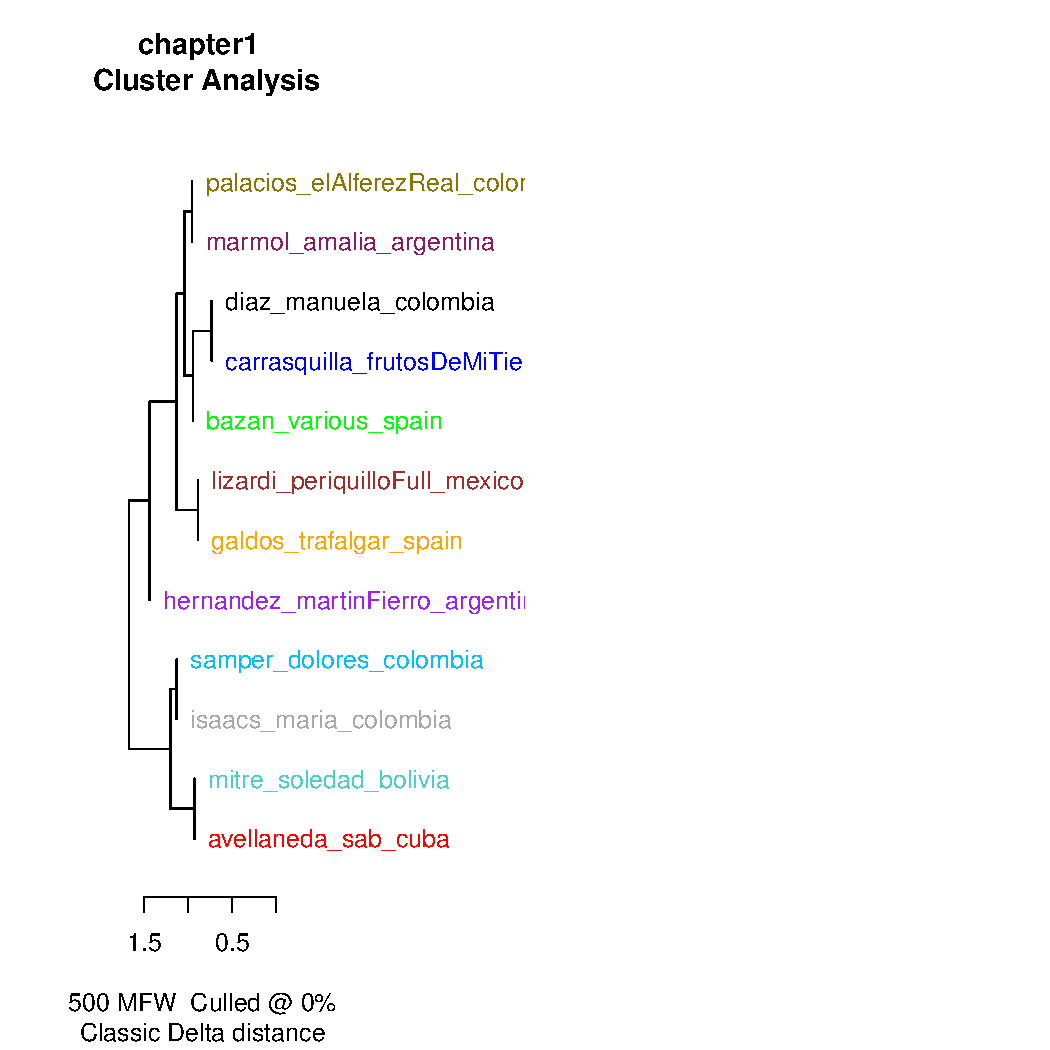
\includegraphics[width=350,height=350]{figure/Figure_1-1} 

\end{knitrout}


Of the many measures for lexical richness outlined by R. Harold Baayen, he maintains that the simple ratio of unique words to total words, or type/token ratio (TTR), is the least informative. 
The reason being that as texts get longer, the addition of new words slows, therefore TTR is not equally representative in texts of varying lengths. 
Baayen discusses numerous options for better comparison, vocabulary growth rates of same size text chunks and side by side interpolated growth curves (236)\nocite{Baayen2008}.
The last two measures will be addressed later, however despite the less robust comparative strength of TTR from the view of linguistic analysis, it does provide a an effective cursory comparison for the purposes of literary investigation. 
Figure 4 plots the TTR from each novel in the corpus of all Spanish language texts available from Project Gutenberg \cite{Project G}.


Figure 2
\begin{knitrout}
\definecolor{shadecolor}{rgb}{0.969, 0.969, 0.969}\color{fgcolor}\begin{kframe}


{\ttfamily\noindent\bfseries\color{errorcolor}{\#\# Error in file(file, "{}rt"{}): cannot open the connection}}

{\ttfamily\noindent\bfseries\color{errorcolor}{\#\# Error in plot(gutttr[, 2], gutttr[, 3], main = "{}TTR of Gutenberg Spanish Texts"{}, : object 'gutttr' not found}}\end{kframe}
\end{knitrout}


Figure 3
\begin{knitrout}
\definecolor{shadecolor}{rgb}{0.969, 0.969, 0.969}\color{fgcolor}
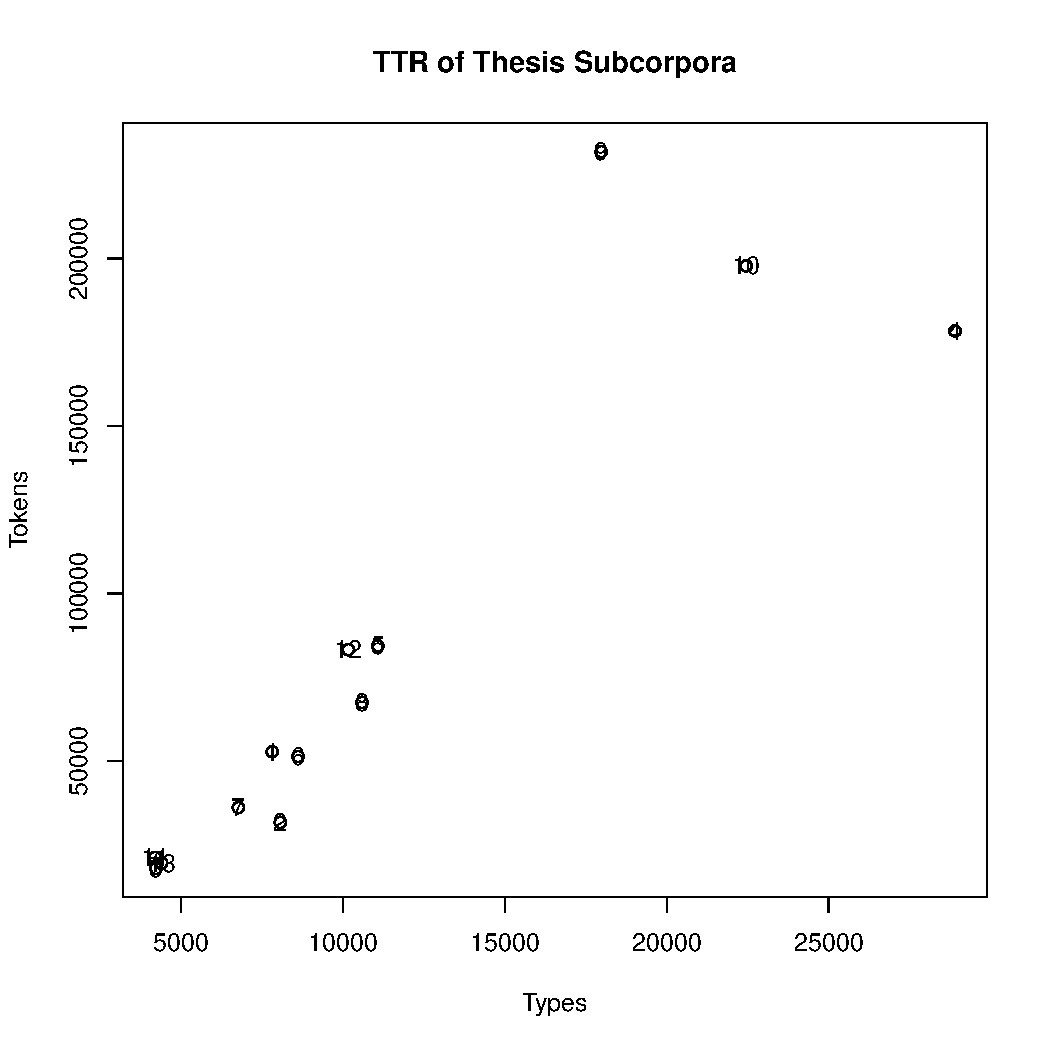
\includegraphics[width=250,height=250]{figure/Figure_3-1} 

\end{knitrout}



Di Paolo chose to highlight the quote denoting \enquote{la gente de ruana} as a class identifying term. It provides an interesting link to the investigation of word choice.
Isaacs uses the word \textit{ruana} six times in his novel, and never with the classist connotation quoted by di Paolo.
Ruana also appears six times in the novel \enquote{El alférez real}, another Colombian work situated in the Cauca Valley that was considerably more successful that Samper's or Carrasquilla's though less so than \textit{María}..
The \textit{Diccionario de la lengua española} from the Real Academia Española list 9 definitions for ruana.
Last on their list, \enquote{especie de capote de monte o poncho} along with the immediately preceding definition \enquote{manta raída}, represent every case of the use by Isaacs.
In the \textit{Corpus del Español}, a collection of 100 million words dating back to the 1200's, the word only appears eleven times and only three times prior to Isaacs novel. \cite{Davies2012}. 
In the RAE's \textit{Corpus de Referencia del Español Actual} the word appears 43 times, over half of which are from Colombia \cite{Crea}.
In their \textit{Corpus Diacrónico del Español} the word appears 54 times, 48 of which are from Colombian sources, see figure 4 for examples \cite{Corde}}.
Interestingly Tomás Carrasquilla holds the place of the largest user of the word.
One might ask why Carrasquilla does not hold the canonical place that Isaacs does?
Answering this question requires looking at far more than a few words, at the overall lexical richness of these novels.
That is to say, of all the words an author chooses to use how many distinct words, or types, do they employ.
It may be possible that a connected readership depends on a certain amount of unique vocabulary that typifies a readers local reality.
However, as a look a lexical richness shows, overly rich vocabulary may have the opposite effect. 


\begin{table}[ht]
\centering
{\tiny
	\caption{Occurences of \textit{ruana} in the RAE's CORDE}
	\label{my-label}
	\begin{tabular}{lllll}
		Casos & Año         & Autor                            & Obra                                                                                    & País      \\
		6     & 1924        & Rivera, José Eustasio            & La vorágine                                                                             & COLOMBIA  \\
		1     & 1911 - 1925 & Suárez, Marco Fidel              & Sueños de Luciano Pulgar, I                                                             & COLOMBIA  \\
		6     & 1867        & Isaacs, Jorge                    & María                                                                                   & COLOMBIA  \\
		22    & 1935 - 1936 & Carrasquilla, Tomás              & Hace tiempos                                                                            & COLOMBIA  \\
		1     & 1932        & Reyles, Carlos                   & El gaucho Florido. La novela de la estancia cimarrona y del gaucho crudo                & URUGUAY   \\
		7     & 1896        & Carrasquilla, Tomás              & Frutos de mi tierra                                                                     & COLOMBIA  \\
		1     & 1626        & Quevedo y Villegas, Francisco de & La vida del Buscón llamado don Pablos                                                   & ESPAÑA    \\
		2     & p 1960      & Buenaventura, Enrique            & A la diestra de Dios Padre                                                              & COLOMBIA  \\
		2     & 1960        & Buenaventura, Enrique            & En la diestra de Dios Padre                                                             & COLOMBIA  \\
		1     & 1956        & Sanín Cano, Baldomero            & Tomás Rueda Vargas. Un humorista y un patriota {[}El oficio de lector{]}                & COLOMBIA  \\
		2     & a 1936      & Nogales Méndez, Rafael           & Memorias                                                                                & VENEZUELA \\
		1     & c 1962      & Isaza de Jaramillo Meza, Blanca  & Itinerario breve                                                                        & COLOMBIA  \\
		1     & 1946 - 1952 & Ballesteros Gaibrois, Manuel     & Historia de América                                                                     & ESPAÑA    \\
		1     & 1673        & Vélez de Guevara, Juan           & Fin de fiesta para la comedia de DQ
		{[}El hidalgo de la Mancha{]} & ESPAÑA   
	\end{tabular}
}
\end{table}



A comparison of the word frequencies of these two novels in Figure 2 helps to emphasize why there would be a broad difference in terms of lexical connection to their readers.
Analysis of the lexicon employed by Isaacs' shows that establishing a stylistic connection is the key to the success of nationally uniting works. 
As the plot shows, there is a tendency for novels to remain below a certain threshold.
For the sixteen novels examined previously through clustering, the mean type/token ration is .1699.
What the shows is that lexical richness may have its limits when it comes to retaining readership. 
Producing connections with readers is achieved by choosing a limited but specific vocabulary.


In order to show some words that Isaacs novel introduced to Colombia's print vernacular, I have gleaned a few words whose print debut is in Isaacs’ novel.
The word list for plotting consists of those words that do not appear in any other text in all Spanish texts available from Project Gutenberg which contain a total of 467,557 unique words.
For this reason it is, to be sure, only a few words are presented here as many words have been eliminated for brevity.
An expanded ngram search of all vocab from the novel will produce many more.
One example is the word hoyuelada, a word that does not appear in the RAE dictionary as an adjective, only as the noun \enquote{hoyuela}.
Nevertheless, Isaacs says of María’s smile \enquote{esa sonrisa hoyuelada era la de la niña de mis amores infantiles} (…).
Other words, such as \enquote{pomarrosos} are less innovative given their botanical nature, but nevertheless curious considering their absence from both the Google Ngram corpora as well as the Corpus del Español until after \textit{Marías} publishing.
This highlights just how important literature was to forming language at the time.
Certainly in colloquial speech the word for this imported fruit tree must have been in existence.
While \textit{pomarrosos} does provided a particularly Colombian example, \textit{chilacoas} does.
Isaacs introduces the word for a regional bird folding neatly into the Romantic reflection of character emotions saying \enquote{oímos de rato en rato el trino melancólico de las chilacoas} (…).
Other biological references such as \textit{espina de mono} have evaded classification and remain in the footnotes of the lastest editions
McGrady calls his manipulation of vocabulary something from \enquote{el Siglo de Oro} noting even complete inventions of words such as \enquote{arrieramente} \cite[43]{McGrady2012}.

\textit{María} spans a gap in historical literary periods, nevertheless it contains typical elements of \textit{romanticismo} and \textit{costumbrismo}.
Some critics even claim that it shows aspects of realism and precursors to \textit{modernismo}.
In fact, Sommer asks if it is possible that the preponderance of love stories in all of the novels she examines is merely a historical phenomenon and not indicative of any underlying pattern of genre.
This makes the need to compare the features of works, apart from genre, exceptionally important.
If thematic features have made novels of a certain genre particularly suited as national allegories, then comparing those novels should present very similar characteristics.
Analyzing their lexical composition should present groupings only along lines of genre.
Instead, as shown in \underline{Figure 1}, the features that may typify a particular genre are less influential than other features that show a distinct grouping than those of critical scholarly intuition.


\section{Solve the problem}

Efraín and María were as impossible a combination as were indigenous and \enquote{colombiano}.
To be sure, the late nineteenth century definition of Colombian was quite narrow, and Isaacs himself found his Jewish heritage to complicate categorizing his identity \cite[160]{Jagoe2003}.
It is Jagoe's examination of \textit{Estudio sobre las tribus indigenas del Magdalena} that helps point out the importance of Isaacs personal experience in examining the role that authorial style plays in unifying nationalist ideologies. 
Jagoe points out that in \textit{Estudios} Isaacs expressed that \enquote{hasta que blancos e indigenas no lleven a cabo un contacto considerable y se mezclen entre si no habran herencias biologicas y culturales que reflejen los distintos pueblos de Colombia} \cite[160]{Jagoe2003}.


Isaacs also makes clear his recognition of the distinguishing role of language in questions of class and race.
As Rama and Pachón have pointed out, class politics of language in former Spanish colonies were no accident and \textit{María} reflects that.
While Isaacs tends to idealize the linguistic stratification of 19th century Colombian society, their inclusion at all emphasizes that the author is making an intentional social commentary.
Isaacs later work on \textit{Estudios} reinforces that fact.
Take as an example the narrator's description of \enquote{la núbil negra} Rufina:
\enquote{Después de haber dejado por tanto tiempo de ver mujeres de esa especie: y lo dejativo de su voz, cuya gracia consiste en gentes de la raza, en elevar el tono en la sílaba acentuada de la palabra final de cada frase} \cite[304]{Isaacs2012}.
Isaacs was not the only observes of changes in intonation distinguishing regionality.
In his \textit{Apuntaciones críticas sobre el lenguaje bogotano}, Rufino José Cuervo quotes D. Eugenio Ochoa saying \enquote{nunca he podido comprender la general manía de convertir en esdrújulos vocablos que nunca lo han sido en castellano} \cite[3]{Cuervo1876}.


The non-standard vocabulary in \textit{Maria} is not a problem of only modern reading, and the earliest editions of the book contained an appendix of vocabulary, classified by region, in which none of the above mentioned words appear.
Isaacs efforts at innovating, while often times antiquated and heavy handed, do not stop with vocabulary.
McGrady points out that the first edition contained uses of \textit{laismo} y \textit{leismo}, practices not common in the Spanish of the Americas.
These were later changed due to critique from Jose Cuervo whose work on the lexicon of the Americas was mentioned previously.


Not all Romance novels from the Americas shared Isaacs tone, and \textit{María} is different in some repects than many other foundational works typically examined alongside the question of national literatures.
\textit{María's} uniqueness was seen by some critics as a redeeming quality, of the ending of the novel Cortázar comments: \enquote{No han sido pocos los que han pensado que \textit{María}, como obra de arte y tratándose del desenlace, supera a las novelas que se le parecen} \cite[57]{Cortazar1908}.
Sommer offers an illuminating counter example to the popularity of \textit{María} and \textit{Sab} in the Argentine novel \textit{Amalia} which she admits \enquote{is read more as a period piece than as a founding text} \cite[111]{Sommer1991}.
Instead \textit{Martín Fierro} by José Hernández became Argentina's national epic because it \enquote{constructed a national voice by appropriating the language of \enquote{authentic} but notoriously shiftless Argentines for patriotic and rational projects} \cite[111]{Sommer1991}.


Many scholars agree that Isaacs manner of addressing the changes in Colombia is through displacing the regional turmoil in his story. 
At one point in history to a certain audience \textit{María} provided an allegory of erotic love, as is the focus of Sommer’s investigation. 
While \textit{María} has been appropriated as iconic nationalist literature, it is less clear that it was intended to be such an allegory of state formation.
What is important to acknowledge is that, as Patiño's insight into Japanese immigration has shown, the novel has served many purposes. 
Still it is shortsighted to say that political climate was not at the forefront of Isaacs mind even if it appears more implicitly in his novel.
For example, McGrady points out phrases such as \enquote{volví a ver ese valle del Cauca, país tan bello caunto desaventurado ya} \cite[314]{McGrady2012}.
He attributes this reference to \enquote{las revoluciones de 1860 a 1863 que asolaron a este estado} \cite[314]{McGrady2012}.
While Isaac's frame of mind is highlighted by political and personal turmoil leading up to María's publication, the novel's importance in Colombian culture has evolved with Colombian society.


In a thematic sense, Isaacs also portrays the act of reading and owning books as a distinguishing feature. 
Unzueta has emphasized the importance of meta-reading in 19th century novels, Isaacs commentary on language itself helps to highlight the distinguishing lexical features such as those found through keyword analysis.
Table 2 (not yet included) lists the words that stand out using the needle in a haystack method.
Many of the words that stand out are borrowings from local indigenous flora and fauna.
This type of examination also finds the stark contrast created by other passages where the literary language is full of \enquote{prácticas todas que no aparecen en el lenguaje normal de Hispanoamérica} \cite[42]{McGrady2012}.
While this contrast parallels social stratification it also may have contributed to the novels success.
The varied regionalism and inclusion of indigenous borrowings facilitated a continually growing readership beyond the initial upper class reaction.

As Franco Moretti indicates the establishment of a work as canonical is driven by popular readership and only later adopted into academia \cite[]{Moretti2013}.
This view places connection through language at the forefront of characteristics that make up a foundational fiction. 
Thus languages frames characters, which are recognized by audiences, who find unity in the imagined constructs of similar experience, and are finally \enquote{folded into the state apparatus} \cite[27]{Felski2008}.

\section{Draw out the implications}
By examining the characteristics of form one may clearly show how authors employ different styles and vocabularies.
How does this show that these styles brought anything to their success or their role in aiding in the imagining of a national community?
It demonstrates that the vocabulary of \enquote{nationalism} is not homogeneous, even under the umbrella of a shared language.
Anderson points out that in Europe \enquote{the lexicographic revolution [...] created and gradually spread, the conviction that languages were, so to speak, the personal property of quite specific groups} \cite[84]{Anderson2006}.
As a consequence these \enquote{groups imagined as communities} felt that they were \enquote{entitled to their autonomous place in a fraternity of equals} \cite[84]{Anderson2006}.
The Spanish colonies provide a unique twist in that, contrary to Europe, each nation already shared a dynastic language-of-state.
For this reason, defining oneself linguistically became an important discussion amongst the elite of the burgeoning republics, a point to which I will return.
For the readers, this linguistic self identification was an important identifying factor for placing themselves in the new broader community, essentially creating a new reality.
Schutz has argued that \enquote{to understand the structure of the literary work as a social construction requires a discriminating concept of reality that has to include various layers} \cite[79]{Embree1998}.
The authorial style that I argue contributes to these novels role in national formation is, for Schutz, the linguistic typification necessary to create an artificial aesthetic reality.
In the case of nationalism, these novels \enquote{symbolized the everyday sphere} while creating the artificial reality of connection between people and places with little else in common.
A uniting artificial reality is precisely the \enquote{imagining} that Anderson attributes with creating national identities. 
Examining the manifestations of linguistic typification, in this case in novels, can only be productive then within their regional frames of reference.


A look at Isaacs relationship to language helps to validate that his awareness of the power of word choice contributed to his writing style which in turn helped to forge his national readership.
Fernando Unzueta summarizes this relationship saying \enquote{reader identification with a text's protagonists, its national contents, and values is crucial to the construction of an imagined community} \cite[82]{Unzueta2002}.
The question of popular reception is less important in connecting \textit{María} to national identity.
However, characteristics that helped Isaacs to be \enquote{institutionalized in the schools and that are now indistinguishable from patriotic histories}, may be the same as those that endeared his novel to the public \cite[add. text]{Sommer1991}.
The foundational fictions of the 19th century can be read through the lens of eroticism, global economy, judaism, etc.
Yet it is the codification of developing national vernaculars for the first time in Spanish American fiction that allowed them to become a part of the public's popular concept of their national culture. 


His ability to combine anachronistic \enquote{castellano} with local dialect and borrowings creates in his novel a mirror of the Colombian linguistic landscape of his time.
At once overly prescriptive and yet steeped in regional variation, language was an important defining factor in the creation of an idependent identity.
The fact these fledgling nations shared a common language with their colonizer as well as with so many neighboring states undergoing independence created a problem in finding solidarity through language.
For this reason Anderson differentiates between the nationalist phenomenon of 19th century and the formation of states along dialectal lines after the loss of Latin as a homogenizing force. 
From a present perspective it becomes apparent that Latin American dialectal variation has a strong significance in ones national identity.
The use of classifying algorithms has helped to show that the early works of literature identified by these geographically defined commuinities showed regional stylistic differences. 
These differences helped to influence a generation of administrators into believing that these popular novels represented a particular national ideal.
The success in their popular acceptance Unzueta points out, \enquote{these texts intended to be thoroughly national, in the characters represented, authors, and audience, and promote self recognition} (100). 
While Isaacs and Galdós were both connecting with a broader audience through their use of language, their preoccupations were quite different.
Isaacs \textit{María} never offers a way forward, but rather continuously laments the loss of past.


One of the largest proponents of using language to promote an independent American identity was Andres Bello \cite[1350]{Gobat2013}. However, as Chapter 3 will explore, the birth of Latin America was far from purely linguistic. Isaacs novel achieved its foundational status by helping Colombians identify as unique in the American context.  Its sentimentalism and scenery helped it to connect readers beyond the Andes. However, there is nothing Latin American about it. Precisely because the construct of Latin America came about in order to establish an elitist identity separate from, but on par with, their counterparts in Europe and the United Sates \cite[1349]{Gobat2013}. According to Michel Gobat a unified resistance to neo-colonial interests was the impetus for the adoption of the concept \cite[1349]{Gobat2013}. The lament in Isaacs' work reveals what Frantz Fanon called the cracks in the edifice of national unity. That is the colonial elite perpetuate national agendas in order to situate themselves in the new national economy. Uniting these continent wide movements under one name in order to resist neo-colonial invasion is the macro version of regional oppression. Isaacs latent defense of regionalism through his novel mirrors his conflicted feelings about the effectiveness of central authority in Colombia. 

%\makeworkscited

\end{document}
